% Präambel
\documentclass[11pt,			% Schriftgröße
a4paper,						% Papierformat
oneside, 						% einseitiges (oneside) oder zweiseitiges (twoside) Dokument
listof=totoc, 					% Tabellen- und Abbildungsverzeichnis ins Inhaltsverzeichnis
bibliography=totoc,				% Literaturverzeichnis ins Inhaltsverzeichnis aufnehmen
titlepage, 						% Titlepage-Umgebung statt \maketitle
headsepline, 					% horizontale Linie unter Kolumnentitel
%abstracton,					% Überschrift beim Abstract einschalten, Abstract muss dazu in {abstract}-Umgebung stehen
DIV18,							% auskommentieren, um den Seitenspiegel zu vergrößern
BCOR6mm,						% Bindekorrektur, die den Seitenspiegel um 6mm nach rechts verschiebt,
cleardoublepage=empty,			% Stil einer leeren eingefügten Seite bei Kapitelwechsel
parskip							% Absatzabstand bei Absatzwechsel einfügen
]{scrbook}			
\usepackage{ucs} 				% Dokument in utf8-Codierung schreiben und speichern
\usepackage[utf8x]{inputenc} 	% ermöglicht die direkte Eingabe von Umlauten
\usepackage[ngerman]{babel} 	% deutsche Trennungsregeln und Übersetzung der festcodierten Überschriften
\usepackage[T1]{fontenc} 		% Ausgabe aller zeichen in einer T1-Codierung (wichtig für die Ausgabe von Umlauten!)
\setlength{\parindent}{0ex} 	% bei neuem Abschnitt nicht einrücken
\linespread{1.2}\selectfont     % Zeilenabstand erhöhen - größere Werte als 1.2 nicht verwenden!!
\usepackage{scrpage2}			% SCR Headings verwenden
\setheadsepline{0.4pt}			% Kopfzeile Linien oben
\setfootsepline{0.4pt}			% Kopfzeile Linien unten
\pagestyle{scrheadings}			% SCR Headings einschalten
\usepackage{graphicx}  			% Einbinden von Grafiken erlauben
\usepackage[format=hang,		% Formatierungen von Unter- / Überschriften
font=normal,
labelfont=bf,
justification=RaggedRight,
singlelinecheck=true,
aboveskip=1mm
]{caption}


% Please add the following required packages to your document preamble:
\usepackage[table,xcdraw]{xcolor}
% If you use beamer only pass "xcolor=table" option, i.e. \documentclass[xcolor=table]{beamer}
% Note: It may be necessary to compile the document several times to get a multi-page table to line up properly
\usepackage{booktabs}
\usepackage{longtable}
\usepackage{pdfpages}



\usepackage{enumitem}			% Erlaubt Änderung der Nummerierung in der Umgebung enumerate

\usepackage{amsmath}			% Ergänzungen für Formeln
\usepackage{textcomp} 			% zum Einsatz von Eurozeichen u. a. Symbolen
\newcommand*\diff{\mathop{}\!\mathrm{d}}	% Differentialzeichen
\newcommand*\Diff[1]{\mathop{}\!\mathrm{d^#1}} % Differentialzeichen höherer Ableitung
\newcommand*\jj{\mathop{}\!\mathrm{j}}	% Komplexe Zahl j

\usepackage[					% Einstellunge Paket hyperref
hyperfootnotes=false			% im pfd-Output Fußnoten nicht verlinken
]{hyperref}

\usepackage{makeidx}			% Paket zur Erstellung eines Index
\usepackage[intoc]{nomencl} 	% zur Erstellung des Abkürzungsberzeichnisses

\usepackage[					% Einstellungen für Fußnoten
bottom,							% Ausrichtung unten
multiple,						% Trennung durch Seperator bei mehreren Fußnoten
hang,
marginal
]{footmisc}

\usepackage{calc}				% Paket zum Berechnen von Längen z.B. 0.8\linewidth

\usepackage{xcolor} 			% einfache Verwendung von Farben in nahezu allen Farbmodellen

\usepackage{listings}			% Darstellung von Quellcode mit den Umgebungen {lstlisting}, \lstinline und \lstinputlisting
\lstset{literate=				% Damit können Umlaute innerhalb Listings geschrieben werden
	{Ö}{{\"O}}1
	{Ä}{{\"A}}1
	{Ü}{{\"U}}1
	{ß}{{\ss}}1
	{ü}{{\"u}}1
	{ä}{{\"a}}1
	{ö}{{\"o}}1
}
\definecolor{mygreen}{rgb}{0,0.6,0}
\definecolor{mygray}{rgb}{0.5,0.5,0.5}
\definecolor{mymauve}{rgb}{0.58,0,0.82}
\lstset{ %
	backgroundcolor=\color{white},   % choose the background color; you must add \usepackage{color} or \usepackage{xcolor}; should come as last argument
	basicstyle=\footnotesize,        % the size of the fonts that are used for the code
	breakatwhitespace=false,         % sets if automatic breaks should only happen at whitespace
	breaklines=true,                 % sets automatic line breaking
	captionpos=t,                    % sets the caption-position to (b) bottom or (t) top
	commentstyle=\color{mygreen},    % comment style
	deletekeywords={...},            % if you want to delete keywords from the given language
	escapeinside={\%*}{*)},          % if you want to add LaTeX within your code
	escapeinside={(*@}{@*)},
	extendedchars=true,              % lets you use non-ASCII characters; for 8-bits encodings only, does not work with UTF-8
	frame=none,	                   	% "single" adds a frame around the code; "none"
	keepspaces=true,                 % keeps spaces in text, useful for keeping indentation of code (possibly needs columns=flexible)
	keywordstyle=\color{blue},       % keyword style
	language=[LaTeX]TeX,             % the language of the code
	morekeywords={*,nomenclature},   % if you want to add more keywords to the set
	numbers=left,                    % where to put the line-numbers; possible values are (none, left, right)
	numbersep=5pt,                   % how far the line-numbers are from the code
	numberstyle=\tiny\color{mygray}, % the style that is used for the line-numbers
	rulecolor=\color{black},         % if not set, the frame-color may be changed on line-breaks within not-black text (e.g. comments (green here))
	showspaces=false,                % show spaces everywhere adding particular underscores; it overrides 'showstringspaces'
	showstringspaces=false,          % underline spaces within strings only
	showtabs=false,                  % show tabs within strings adding particular underscores
	stepnumber=1,                    % the step between two line-numbers. If it's 1, each line will be numbered
	stringstyle=\color{mymauve},     % string literal style
	tabsize=2,	                   % sets default tabsize to 2 spaces
	title=\lstname                   % show the filename of files included with \lstinputlisting; also try caption instead of title
}

\makeindex						% Indexverzeichnis erstellen
\makenomenclature				% Abkürzungsverzeichnis erstellen

% -----------------------------------------------------------------------------------------------------------------
% Zum Aktualisieren des Abkürzungsverzeichnisses (Nomenklatur) bitte auf der Kommandozeile folgenden Befehl aufrufen :
% makeindex <Dateiname>.nlo -s nomencl.ist -o <Dateiname>.nls
% Oder besser: Kann in TexStudio unter Tools-Benutzer als Shortlink angelegt werden
% Konfiguration unter: Optionen-Erzeugen-Benutzerbefehle: makeindex -s nomencl.ist -t %.nlg -o %.nls %.nlo
% -----------------------------------------------------------------------------------------------------------------

% Hier die persönlichen Daten eingeben:

\newcommand{\titel}{BlindControl}
\newcommand{\untertitel}{Eine smarte Steuerung für Jalousien}
\newcommand{\arbeit}{Projektdokumentation}
\newcommand{\studiengang}{Elektrotechnik}
\newcommand{\studienrichtung}{Fahrzeugelektronik}
\newcommand{\studienschwerpunkt}{}
\newcommand{\autor}{Maximilian Bachmann, Marvin Eisenmann, Florian Vetter}
\newcommand{\matrikelnr}{123 456}
\newcommand{\kurs}{TFE17-2}
\newcommand{\firma}{Firma (Angabe entfällt ggf. bei Studienarbeit)}
\newcommand{\abgabe}{30.04.2019}
\newcommand{\betreuerdhbw}{Hans Juergen Herpel}
\newcommand{\betreuerfirma}{Gutachter der Firma (Angabe entfällt ggf. bei Studienarbeit)}
\newcommand{\jahr}{2019}			% für Angabe im Copyright-Vermerk der Titelseite

% Folgende Zeilen definieren Abkürzungen, um Befehle schneller eingeben zu können
\newcommand{\ua}{\mbox{u.\,a.\ }}
\newcommand{\zB}{\mbox{z.\,B.\ }}
\newcommand{\bs}{$\backslash$}

% Folgende Zeilen weden benötigt, um Tikz und PGF-Plot-Grafiken einzubinden
\usepackage{pgfplots}
\usepackage{pgfplotstable}
\pgfplotsset{compat=newest}
\usepgfplotslibrary{smithchart}
\usepackage{tikz}						% Tikz sollte nach Listings Pakete geladen werden.
\usetikzlibrary{arrows}

\hyphenation{Schrift-ar-ten}


% -------------------------------------------------------------------------------------------
%                     Beginn des Dokumenteninhalts
% -------------------------------------------------------------------------------------------
\begin{document}
\setcounter{secnumdepth}{3}				% Nummerierungstiefe fürs Inhaltsverzeichnis
\setcounter{tocdepth}{3}
\sffamily								% für die Titelei serifenlose Schrift verwenden

% ------------------------------ Titelei -----------------------------------------------------

\thispagestyle{plain}
\begin{titlepage}
\enlargethispage{4.0cm}
\sffamily 								% Serifenlose Grundschrift für die Titelseite einstellen

\parbox{0.5\linewidth}{
\begin{flushleft}
% Hier ggf. ein Logo der Firma
\end{flushleft}
}
\parbox{0.5\linewidth}{
\begin{flushright}
	\includegraphics[width=0.4\linewidth]{images/DHBW_d_R_FN_46mm_4c}\\[5ex]
\end{flushright}
}
				

\begin{center}

\huge{\textsc{\textbf{\titel}}}\\[1.5ex]
\Large{\textbf{\untertitel}}\\[5ex]
\LARGE{\textbf{\arbeit}}\\[2ex]
%\normalsize{für die Prüfung zum\\[1ex] Bachelor of Engineering}\\[3ex]
\Large{Studiengang \studiengang}\\[2ex]
\large{Studienrichtung \studienrichtung}\\[1ex]
%\large{ \studienschwerpunkt}\\[2ex]
\normalsize{Duale Hochschule Baden-Württemberg Ravensburg, Campus Friedrichshafen}\\[5ex]
von\\[1ex] \autor \\[20ex]


\end{center}

\begin{flushleft}

\begin{tabular}{ll}
Abgabedatum:					& \quad \abgabe \\
Bearbeitungszeitraum:		   		& \quad 07.01.2019 - 07.03.2019   \\ 
%Matrikelnummer: 			& \quad \matrikelnr \\ 
Kurs: 							& \quad \kurs \\
%Ausbildungsfirma:	 			& \quad \firma \\ 
%Betreuer der Ausbildungsfirma:  & \quad \betreuerfirma \\ 
%Gutachter der Dualen Hochschule: & \quad \betreuerdhbw \\ [5ex]

\end{tabular} 



\small
Copyrightvermerk:\\

Dieses Werk einschließlich seiner Teile ist \textbf{urheberrechtlich geschützt}. Jede Verwertung außerhalb der engen Grenzen des Urheberrechtgesetzes ist ohne Zustimmung des Autors unzulässig und strafbar. Das gilt insbesondere für Vervielfältigungen, Übersetzungen, Mikroverfilmungen sowie die Einspeicherung und Verarbeitung in elektronischen Systemen.
\end{flushleft}
\begin{flushright}
\copyright{} \jahr
\end{flushright}
\end{titlepage}

\cleardoublepage 				% erzeugt die Titelseite
\pagenumbering{roman}					% kleine, römische Seitenzahlen für Titelei
%%% Ggf. folgende Zeile auskommentieren, falls der Sperrvermerk gewünscht ist.
%\chapter*{Sperrvermerk} %*-Variante sorgt dafür, das der Sperrvermerk nicht im Inhaltsverzeichnis auftaucht
%gemäß Ziffer 1.1.13 der Anlage 1 zu §§ 3, 4 und 5  der Studien- und Prüfungsordnung für die Bachelorstudiengänge im Studienbereich Technik der Dualen Hochschule Baden-Württemberg vom 29.09.2017 in der Fassung vom 25.07.2018:
%
%Der Inhalt dieser Arbeit darf weder als Ganzes noch in Auszügen Personen außerhalb des Prüfungsprozesses und des Evaluationsverfahrens zugänglich gemacht werden, sofern keine anders lautende Genehmigung vom Dualen Partner vorliegt.
%
%Musterstadt, den \today \\[4ex]
%
%\rule[-0.2cm]{5cm}{0.5pt} \\
%
%\textsc{\autor} \\[10ex]

\chapter*{Erklärung} %*-Variante sorgt dafür, dass die Erklärung nicht im Inhaltsverzeichnis auftaucht

gemäß Ziffer 1.1.13 der Anlage 1 zu §§ 3, 4 und 5  der Studien- und Prüfungsordnung für die Bachelorstudiengänge im Studienbereich Technik der Dualen Hochschule Baden-Württemberg vom 29.09.2017 in der Fassung vom 25.07.2018.

Ich versichere hiermit, dass ich meine Bachelorarbeit (bzw. Projektarbeit oder Studienarbeit bzw. Hausarbeit) mit dem Thema:

\begin{quote}
	\textit{\titel} -\textit{ \untertitel }
\end{quote}

selbstständig verfasst und keine anderen als die angegebenen Quellen und Hilfsmittel benutzt habe. Ich versichere zudem, dass die eingereichte elektronische Fassung mit der gedruckten Fassung übereinstimmt.\\[10ex]

Musterstadt, den \today \\[4ex]

\rule[-0.2cm]{5cm}{0.5pt} \\

\textsc{\autor} \\[10ex]

\cleardoublepage 				% Einbinden der eidestattlichen Erklärung
%\chapter*{Kurzfassung} %*-Variante sorgt dafür, das Abstract nicht im Inhaltsverzeichnis auftaucht

Text Kurzfassung

\cleardoublepage
   			% Einbinden des Abstracts

\tableofcontents						% Erzeugen des Inhalsverzeichnisses
\cleardoublepage

% --------------------------------------------------------------------------------------------
%                    Inhalt der Bachelorarbeit
%---------------------------------------------------------------------------------------------
\pagenumbering{arabic}					% arabische Seitenzahlen für den Hauptteil

\rmfamily

\chapter{Einführung}
\label{cha:Einführung}
Das Projekt BlindControl entstand im Rahmen der Mikrocontroller Vorlesung des Dozenten Hans Jürgen Herpel an der DHBW Ravensburg Campus Friedrichshafen. Ziel ist es, eine Projektentwicklung anhand eines selbstgewählten Beispiels zu durchlaufen, um die entsprechenden Vorgänge zu erlernen und zu dokumentieren. Das fertige Projekt kann in dem zugehörigen \href{https://github.com/maxbachmann/BlindControl}{Git Repository} auf Github angesehen und verwendet werden. Zudem gibt es zu dem Projekt ein ausführliches \href{https://github.com/maxbachmann/BlindControl/wiki}{Github Wiki}.

% Was ist das Problem?
\section{Heranführung an die Problemstellung}
Die dem Projekt zugrundeliegende Idee ist die automatische Ansteuerung einer Jalousie mittels Home Assistant. Viele Jalousien sind nur manuell zu steuern oder nur mit teurer Technik automatisiert. Dennoch birgt eine automatische Steuerung einen hohen Comfort, auf den auch andere Anwender nicht verzichten sollten. Anwendungsbeispiele sind Folgende:
\begin{itemize}
	\item Bei zu hoher Sonneneinstrahlung verdunkelt die Jalousie automatisch, um eine angenehme Raumtemperatur auch im Sommer zu wahren.
	\item Jalousien sind durch ihren Aufbau sehr windanfällig und können leicht Schaden nehmen, oder gar anwesende Personen gefährden, sollte ein Sturm aufziehen. Auch hier kann eine Steuerung reagieren und die Jalousien automatisiert hochfahren und so zu schützen.
	\item Zusätzlich zu der automatisierten Steuerung kann es auch vorkommen, dass ein Nutzer beispielsweise auf dem Sofa liegt und durch die Sonnen geblendet wird. Um nicht aufstehen und zum Schalter an der Wand laufen zu müssen, könnte eine Heimautomatisierung zum Einsatz kommen, in der eine manuelle Steuerung der Jalousien integriert ist. Damit könnten diese mit dem Smartphone, das viele Benutzer immer bei sich haben, gesteuert werden.
	\item Auch die nachträgliche Installation solcher Technik kann Probleme bereiten, wenn beispielsweise Leitungen von der Jalousie zu dem Steuerungsserver gelegt werden müssen. Dagegen ist eine auf Funk basierte Kommunikation der einzelnen Komponenten optimal.
\end{itemize}
Auf Grundlage der genannten Anwendungssituationen wurden für das Projekt BlindControl die Anforderungen(Requirements) entworfen, sowie die Hardware und Software ausgewählt.

% Wie sieht der Lösungsraum aus?
\section{Lösungsansätze}
Um alle genannten Funktionen und Eigenschaften zusammen nutzen zu können, wird eine zentrale Steuereinheit benötigt, die alle Jalousien verwaltet. Auf diese sollte der Benutzer zugreifen können, um die manuelle Steuerung zu übernehmen. Zudem sollten hier alle Befehle an die Jalousien zentral gesendet werden, die damit eine eigene Ansteuerung brauchen. Um auf Umwelteinflüsse, wie Wind und Helligkeitswert zu reagieren. Dafür wird ein Sensor-Modul gebraucht, um die Steuereinheit auch dezentral platzieren zu können. Das gesamte System sollte möglichst einfach installierbar und anpassbar sein, sowie durch Funkbetrieb Kabelleitungen zwischen den Untersystemen vermeiden und eine einfache Einrichtung gewährleisten.

% Welche Lösung wurde gewählt?
Um ein eben beschriebenes System zu gewährleisten, wurde das System in drei Untersysteme gegliedert. Die Zentralsteuerung wurde mit einem Raspberry Pi 3 realisiert, der mit Raspbian Stretch aufgesetzt wurde und mit HomeAssistant als Smarthome Verwaltung konfiguriert wurde. Um eine schnelle Software Installation zu garantieren, wurde ein Ansible Skript eingesetzt. Zusätzlich wurde Unbound für eine privatere DNS Abfrage installiert. Die Sensorwerte wurden über einen Nordic Mikrocontroller eingelesen und über ein Thread Netzwerk an den Border Router mittels MQTT übermittelt. Dieser konnte dann auf Grund dieser Daten mittels MQTT einen ESP32 Befehle zum Jalousien Stand senden.
\chapter{Grundlagen}
\label{cha:Grundlagen}

\section{MQTT (Message Queue Telemetry Transport)}

\subsection{Allgemein}
Bei MQTT\nomenclature{MQTT}{Message Queue Telemetry Transport} handelt es sich um ein einfaches TCP/IP basiertes Nachrichtenprotokoll, das auf den Bereich Mobile und Internet of Things (IoT) zugeschnitten ist. MQTT ist gerade im Bereich der Heimautomatisierung sehr beliebt.

Ziele von MQTT sind neben einer hohen Zuverlässigkeit ein sparsamer Umgang mit Bandbreite und Ressourcen. Dadurch eignet sich MQTT auch zur Kommunikation mit mobilen Geräten, bei denen Bandbreite und Ressourcen knapp sind.

\subsection{Publish/Subscribe Verfahren}
Der Nachrichtenaustausch bei MQTT funktioniert über das Publish/Subscribe Verfahren. Bei Publish/Subscribe kommuniziert der Sender der Nachricht nicht direkt mit dem Empfänger, sondern wendet sich an einen Broker, welcher die Zustellung der Nachricht übernimmt. Der Broker entkoppelt so den Sender vom Empfänger der Nachrichten.

\subsection{MQTTS (Message Queue Telemetry Transport Secure)}
Bei MQTTS\nomenclature{MQTT}{Message Queue Telemetry Transport Secure} wird die Kommunikation mit TLS/SSL verschlüsselt. Damit wird ein Abhören der Nachrichten erschwert.

\section{TLS (Transport Layer Security)}
TLS\nomenclature{TLS}{Transport Layer Security} (Vorgänger SSL[Secure Sockets Layer])\nomenclature{SSL}{Secure Sockets Layer} ist ein Verschlüsselungsprotokoll zur Verschlüsselung einer Kommunikation. Zu Beginn werden die Zertifikate zwischen zwei Kommunikationspartnern mittels eines public key ausgetauscht. Dabei identifizieren sich beide nacheinander, bevor dann eine verschlüsselte Verbindung aufgebaut ist.


\section{ESP32}
Der ESP32 wird von Espressif hergestellt und besitzt ein schon eingebautes WLAN/Bluetooth Modul. Damit kann er entweder ein eigenes WLAN\nomenclature{WLAN}{Wireless Local Area Network} Netzwerk aufbauen, oder mit einem vorhandenen Netzwerk kommunizieren, ohne zusätzliche Shields zu benötigen, wie ein Arduino. Der Mikrocontroller kann mit entsprechenden Librarys in der Arduino IDE programmiert werden, oder in der ESP IDF Umgebung\footnote{siehe Kapitel~\ref{cha:Installation_IDF}}.

Abbildung~\ref{fig:esp32} zeigt den Aufbau eines ESP32. Auf der linken Seite sind alle kompatiblen Protokolle für die Pins aufgelistet. Interessant ist dabei auch, dass der ESP32 zwei Cores besitzt mit denen zwei Tasks gleichzeitig ausgeführt werden können. Dadurch wird Multi Threading möglich. Zusätzlich ist der Mikrocontroller mit einem Ultra Low Power Coprocessor ausgestattet, wodurch ein sehr stromsparender Betrieb möglich wird. Damit ist der ESP32 perfekt für IoT Anwendungen geeignet.

\begin{figure}[hbt]
	\centering
	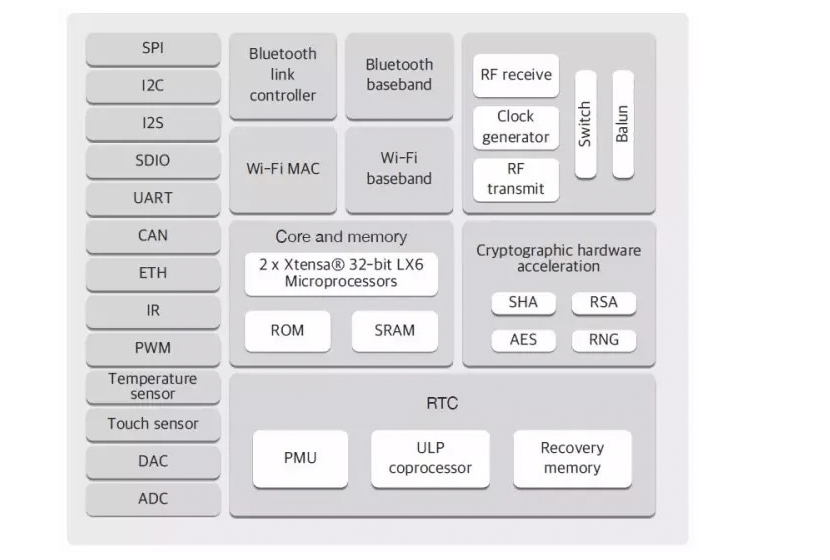
\includegraphics[width=0.7\linewidth]{images/esp32}
	\caption[ESP32 Aufbau]{Aufbau eines ESP32.}
	\label{fig:esp32}
\end{figure}

\chapter{Anforderungen}
\label{cha:Anforderungen}

% Tabelle Requirements
% UseCase(s)

\section{Requirements}
Die Anforderungen an gesamte System wurden in Requirements geschrieben. Zusätzlich dazu wurde für Jedes eine Kategorie festgelegt, für die es gilt.

\textit{Kategorie:} \textbf{F}(Funktional); \textbf{IF}(Interface);
 \textbf{Q}(Quality)\\
\textit{Verifikationsmethode:} \textbf{S}(Similaris); \textbf{I}(Inspektion); 
\textbf{R}(Review); \textbf{M}(Measurement);
\textbf{A}(Analysis); \textbf{T}(Test)
%Kategorie:
%\begin{itemize}
%	\item F = Funktional
%	\item IF = Interface
%	\item Q = Quality
%\end{itemize}
%Verifikationsmethode:
%\begin{itemize}
%	\item S(imiliaris)
%	\item I(nspection)
%	\item R(eview)
%	\item M(easurement)
%	\item A(nalysis)
%	\item T(est)
%\end{itemize}


% Please add the following required packages to your document preamble:
% \usepackage{booktabs}
% \usepackage[table,xcdraw]{xcolor}
% If you use beamer only pass "xcolor=table" option, i.e. \documentclass[xcolor=table]{beamer}
% \usepackage{longtable}
% Note: It may be necessary to compile the document several times to get a multi-page table to line up properly
\begin{longtable}[ht]{p{0.03\textwidth}  p{0.8\textwidth} p{0.04\textwidth} p{0.04\textwidth}}
	
	\toprule
	\rowcolor[HTML]{FFFC9E} 
	{\color[HTML]{333333} \textbf{Nr.}} & {\color[HTML]{333333} \textbf{Beschreibung}}  & {\color[HTML]{333333} \textbf{Kat.}} & {\color[HTML]{333333} \textbf{VM}} \\* \midrule
	\endfirsthead
	%
	\multicolumn{4}{c}%
	{{\bfseries Table \thetable\ continued from previous page}} \\
	\toprule
	\rowcolor[HTML]{FFFC9E} 
	{\color[HTML]{333333} \textbf{Nr.}} & {\color[HTML]{333333} \textbf{Beschreibung}}  & {\color[HTML]{333333} \textbf{Kat.}} & {\color[HTML]{333333} \textbf{VM}} \\* \midrule
	\endhead
	%
	1 & Das System soll modular in einen Regler, ein Sensormodul und eine Aktorsteuerung aufgeteilt sein                                                                                                                                                                                          & F & T \\* \midrule
	2 & Das System soll die Position einer Jalousie zwischen 0\% und 100\% einstellen können                                                                                                                                          & F& T                                   \\* \midrule
	3 & Der Sollwert für die Jalousieposition soll mit Home Assistant (Smarthome Plattform) manuell einstellbar sein                                                                                                & IF & T                                  \\* \midrule
	4 & Der Sollwert für die Jalousieposition soll eine Schnittstelle zur manuellen Einstellung der Jalousieposition bieten sein                                                                                                                                    & IF& T                                   \\* \midrule
	5 & Der Sollwert für die Jalousieposition soll entsprechend der Helligkeit einstellbar sein                                                                                                                                      & IF& T                                   \\* \midrule
	6 & Der Sollwert für die Jalousieposition soll entsprechend der Windstärke einstellbar sein                                                                                                                                    & IF& T                                   \\* \midrule
	7 & Das System soll aktuelle Sensorwerte ausgeben                                                                                                                                  & IF& T                                   \\* \midrule
	8 & Das System soll die neue Jalousieposition ausgeben                                                                                                                                       & IF& T                                   \\* \midrule
	9 & Die aktuelle Helligkeit soll mit Homeassistant angezeigt werden können                                                                                                                                 & IF& T                                   \\* \midrule
	10 & Die aktuelle Windstärke soll mit Homeassistant angezeigt werden können                                                                                                                                    & IF& T                                   \\* \midrule
	11 & Die neue Jalousieposition soll mit Homeassistant angezeigt werden können 	                                                                                                                                     & IF& T                                   \\* \midrule
	12 & Das Sensormodul soll netzunabhängig betrieben werden.                                                                                                                                  & F& I                                   \\* \midrule
	13 & Die Batterie des Sensormoduls soll mindestens 1 Jahr überdauern                                                                                                                                     & F& T                                   \\* \midrule
	14 & Die Batterie des Sensormoduls soll austauschbar sein                                                                                                                                      & F& I                                  \\* \midrule
	15 & Das System soll 1 mal pro Sekunde aktualisiert werden                                                                                                                                      & F& T                                   \\* \midrule
	16 & Das System (bis auf das Sensormodul) soll über eine externe Spannungsversorgung betrieben werden                                                                                                                                     & F& T                                   \\* \midrule
	17 & Die aktuellen Sensorwerte sollen vom Sensormodul gemessen werden                                                                                                                                      & IF& T                                   \\* \bottomrule
\end{longtable}

\section{UseCase}
Die Abbildung~\ref{fig:UseCase} zeigt den normalen Anwendungsfall des Systems. Der Benutzer kann Einfluss auf die Jalousie Software nehmen, mittels HomeAssistent. Von diesem aus gehen die Befehle an den Regler und es werden aktuelle Informationen an die Statusanzeige gesendet. Der Regler wiederum entscheidet, ob eine Handlung nötig wird und kann dementsprechend Befehle an den Aktor senden, der den Motor der Jalousie steuert. Er kann auch seinen aktuellen Status an die Statusanzeige senden. Außer dem Benutzer kann zusätzlich eine Wartungsperson direkt auf die Jalousie Steuerung zugreifen und änderungen vornehmen.
\begin{figure}[hbt]
	\centering
	\includegraphics[width=1\linewidth]{images/UseCase}
	\caption[UseCase Diagramm]{UseCase Diagramm für den normalen Anwendungsfall.}
	\label{fig:UseCase}
\end{figure}
\chapter{Planung des Projekts}
\label{cha:Planung}

\section{Arbeitspakete}

Es bietet sich an das Projekt in mehrere Arbeitspakete aufzuteilen. Hierzu bietet es sich an sich an den verwendeten Codemodulen zu orientieren. Dies sind in diesem Projekt das Regler Module, Das Actuator Module, das Sensor Module und Codeteile wie der Wifi-Task\nomenclature{Wifi}{Wireless Fidelity} die für mehrere Code Module in gleicher Form benötigt werden. Innerhalb der größeren Module Actuator Module und Sensor Module bietet es sich an eine weiter Unterteilung entsprechend der Tasks vorzunehmen. Die Grafik \ref{fig:arbeitspakete} zeigt die genaue Aufteilung der Arbeitspakete.

\begin{figure}[hbt]
	\centering
	\includegraphics[width=1\linewidth]{images/arbeitspakete}
	\caption[Arbeitspakete]{Arbeitspakete}
	\label{fig:arbeitspakete}
\end{figure}

\section{Zeitplan}
Das Grafik \ref{fig:time_plan} zeigt den Zeitbedarf für die einzelnen Arbeitspakete in Form eines Gant Diagramms. Der Zeitbedarf für die einzelnen Arbeitspakete kann ebenfalls aus der Grafik \ref{fig:arbeitspakete} abgelesen werden.

\begin{figure}[hbt]
	\centering
	\includegraphics[width=1\linewidth]{images/Gant}
	\caption[Zeitplanung als Gant Diagramm]{Zeitplanung als Gant Diagramm}
	\label{fig:time_plan}
\end{figure}


\section{Kostenschätzung}
\label{cha:Planung_cost}
In der Planungsphase wurde angenommen, dass mit anderen Mikrocontrollern und damit einem höheren Aufwand gearbeitet wird. Damit ergeben sich gesamt 2200 SLOC\nomenclature{SLOC}{Source Lines Of Code}. Die Vorlesung Mikrocontroller umfasst 64h und somit ergibt sich im Schnitt 34 lines/h, die geschrieben werden müssen. Die Kostenschätzung nach COCOMOII\_2000.4 ist in Abbildung~\ref{fig:cost_plan} zu sehen.

\begin{figure}[hbt]
	\centering
	\includegraphics[width=1\linewidth]{images/cost_plan_img}
	\caption[Kostenschätzung Planung]{Kostenschätzung bei der Planung.}
	\label{fig:cost_plan}
\end{figure}
\chapter{Architektur}
\label{cha:Architektur}

\section{Statische Architektur}
% mit Component diagramm

\section{Verhalten}
% mit state or Activity Diagram


Die Abbildung %\ref{fig:Sequence_UseCase} zeigt die Kommunikation zwischen den einzelnen Modulen mithilfe von MQTTS. Die Darstellung der Kommunikation ist zur besseren Übersicht hierbei auf das minimum reduziert. Das Regler Modul dient zur Verwaltung aller Steuerungsinputs. Es kann sich hierbei sowohl um Inputs von Sensor Modulen, als auch um eine manuelle Ansteuerung handeln, die beispielsweise über eine Sprachsteuerung erfolgt. Auf Basis dieses Inputs entscheidet es welche Position die Jalousie anfahren soll. Die Anzahl an Sensor Modulen und Modulen die eine manuelle Ansteuerung vornehmen ist hierbei nicht begrenzt. Die anzusteuernde Position wird von dem Regler Modul wieder auf das entsprechende topic (message identifier) gesendet und kann anschließend von einer beliebigen Anzahl an Aktor Modulen ausgelesen werden.

Da der ESP32 über zwei Kerne verfügt und zudem bereits mit FreeRTOS ausgeliefert wird und dadurch über einen Scheduler verfügt, bietet sich die Nutzung von Tasks an. Zur Darstellung der Funktionsweise werden daher auch hier Sequenzdiagramme genutzt, die die Kommunikation zwischen den einzelnen Tasks zeigt. Abbildung \ref{fig:Sequence_UserInput} zeigt die Ansteuerung des Aktormoduls. Bei dem User handelt es sich in diesem Fall um das Regler Modul, welches die neue Position mithilfe von MQTTS verschlüsselt überträgt. Der MQTT Task liest die neue Position aus, prüft ob diese zwischen 0 und 100 Prozent liegt und überschreibt die alte Position in einer Queue der Größe 1. Der Motor Control Task liest die neue Position aus der Queue aus, steuert den Motor der Jalousie an um die entsprechende Position zu erreichen und speichert die neue Position anschließend im Flash des ESP32 um diese auch nach einem Neustart wieder abrufen zu können. Dennoch kann nicht ausgeschlossen werden, dass aufgrund eines Fehlers die aktuelle Position nicht mit der gespeicherten Position übereinstimmt. Dies hat zur Folge, dass die Jalousie außerhalb des vorgesehen Bereichs von 0-100 Prozent angesteuert wird und dadurch Schaden nimmt. Um dies zu verhindern macht es Sinn an den Bereichsenden, also bei 0 Prozent und 100 Prozent einen Endstopp einzusetzen.
Abbildung \ref{fig:SequenceMotorControl} zeigt die Implementierung der Endstopps. Der Interrupt Task wird ausgeführt wenn ein Endstopp erreicht wird. Dieser schreibt die Information welcher Interrupt getriggert wurde in eine Queue der Größe 10, so dass auch mehrere Interrupts abgespeichert und dann sequentiell abgearbeitet werden können. Der GPIO Task ist ein Task der die Interrupts aus der Queue ausliest. Handelt es sich um einen Interrupt von einem Endstopp löscht er den Motor Control Task um so zu verhindern, dass dieser den Motor weiter außerhalb des vorgesehenen Bereichs ansteuert. Anschließend korrigiert er die aktuelle Position der Jalousie und speichert diese wieder im Flash ab. Nach der Korrektur erstellt er den Motor Control Task neu, so dass dieser die Position wieder entsprechend des Inputs ansteuern kann. Ein weitere Anforderung ist es auch beim Endkunden noch auf sicherem Weg Updates auf das Endgerät einspielen zu können. Abbildung \ref{fig:Sequence_Update} zeigt wie ein entsprechendes Update erfolgt. Hierbei werden zunächst Updateinformation von einem Webserver geladen. Diese beinhalten die Information welche Version der Anwendung am Aktuellsten ist und auf welchem Server diese sich befinden. Ist die Version der aktuellsten Version neuer als die aktuell eingesetzte Version, wird diese heruntergeladen. Der ESP32 startet anschließend mit der neuen Version neu. Scheitert dies fällt er zurück auf die alte Softwareversion. Zur Absicherung der Verbindung wird hierbei tls Verschlüsselung eingesetzt. Weiterhin ist es nicht möglich einen falschen Updateserver anzugeben, da dieser lokal auf dem Gerät hinterlegt ist und durch Secure Boot in Verbindung mit Flash Encryption kann auch ein lokales Einspielen anderer Software, sowie das Auslesen von Informationen wie WLAN Passwörtern wirkungsvoll verhindert werden. Damit bleibt nur die Möglichkeit die Updateinformationen direkt auf dem Server zu manipulieren. Standardmäßig werden OTA Updates mit MD5 gehasht, was nicht mehr als sicher gilt. Für eine Endanwendung wäre es daher sinnvoll stattdessen besipielsweise sha256 zu nutzen. Die vorliegende Implementierung macht hiervon aktuell jedoch keinen Gebrauch. Weiterhin ist die Sicherheit durch die genannten Sicherheitsvorkehrungen bedeutend höher als bei den aktuell üblichen IOT Geräten.

%\begin{figure}[hbt]
%	\centering
%	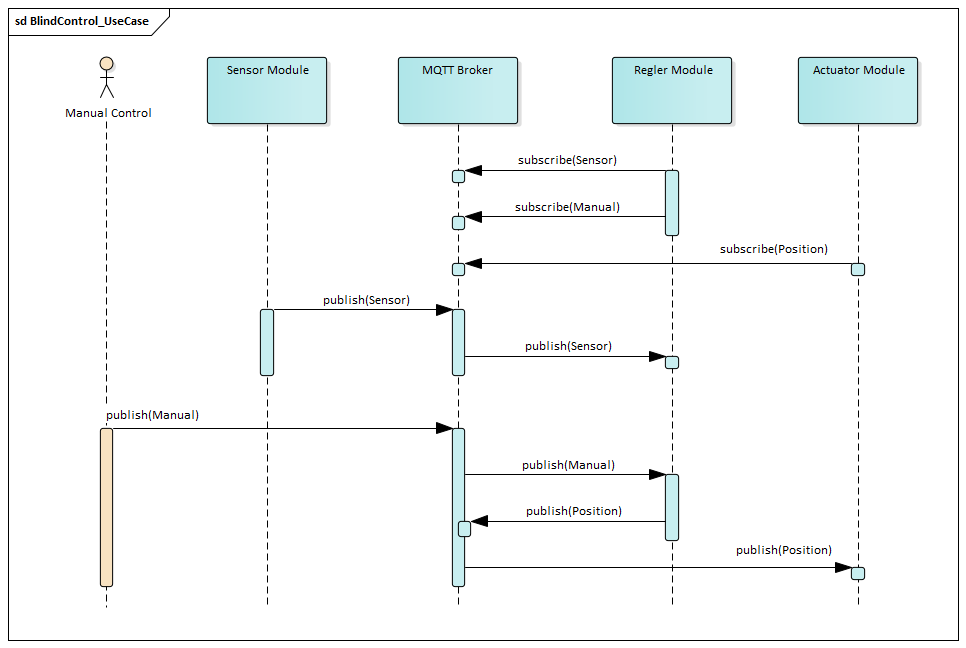
\includegraphics[width=1\linewidth]{images/Sequence_UseCase}
%	\caption[Sequence_UseCase]{Sequenz Diagramm für die Kommunikation zwischen den einzelnen Modulen}
%	\label{fig:Sequence_UseCase}
%\end{figure}

\begin{figure}[hbt]
	\centering
	\includegraphics[width=1\linewidth]{images/Sequence_UserInput}
	\caption[Sequence UserInput]{Sequenz Diagramm für die Ansteuerung des Aktormoduls}
	\label{fig:Sequence_UserInput}
\end{figure}

\begin{figure}[hbt]
	\centering
	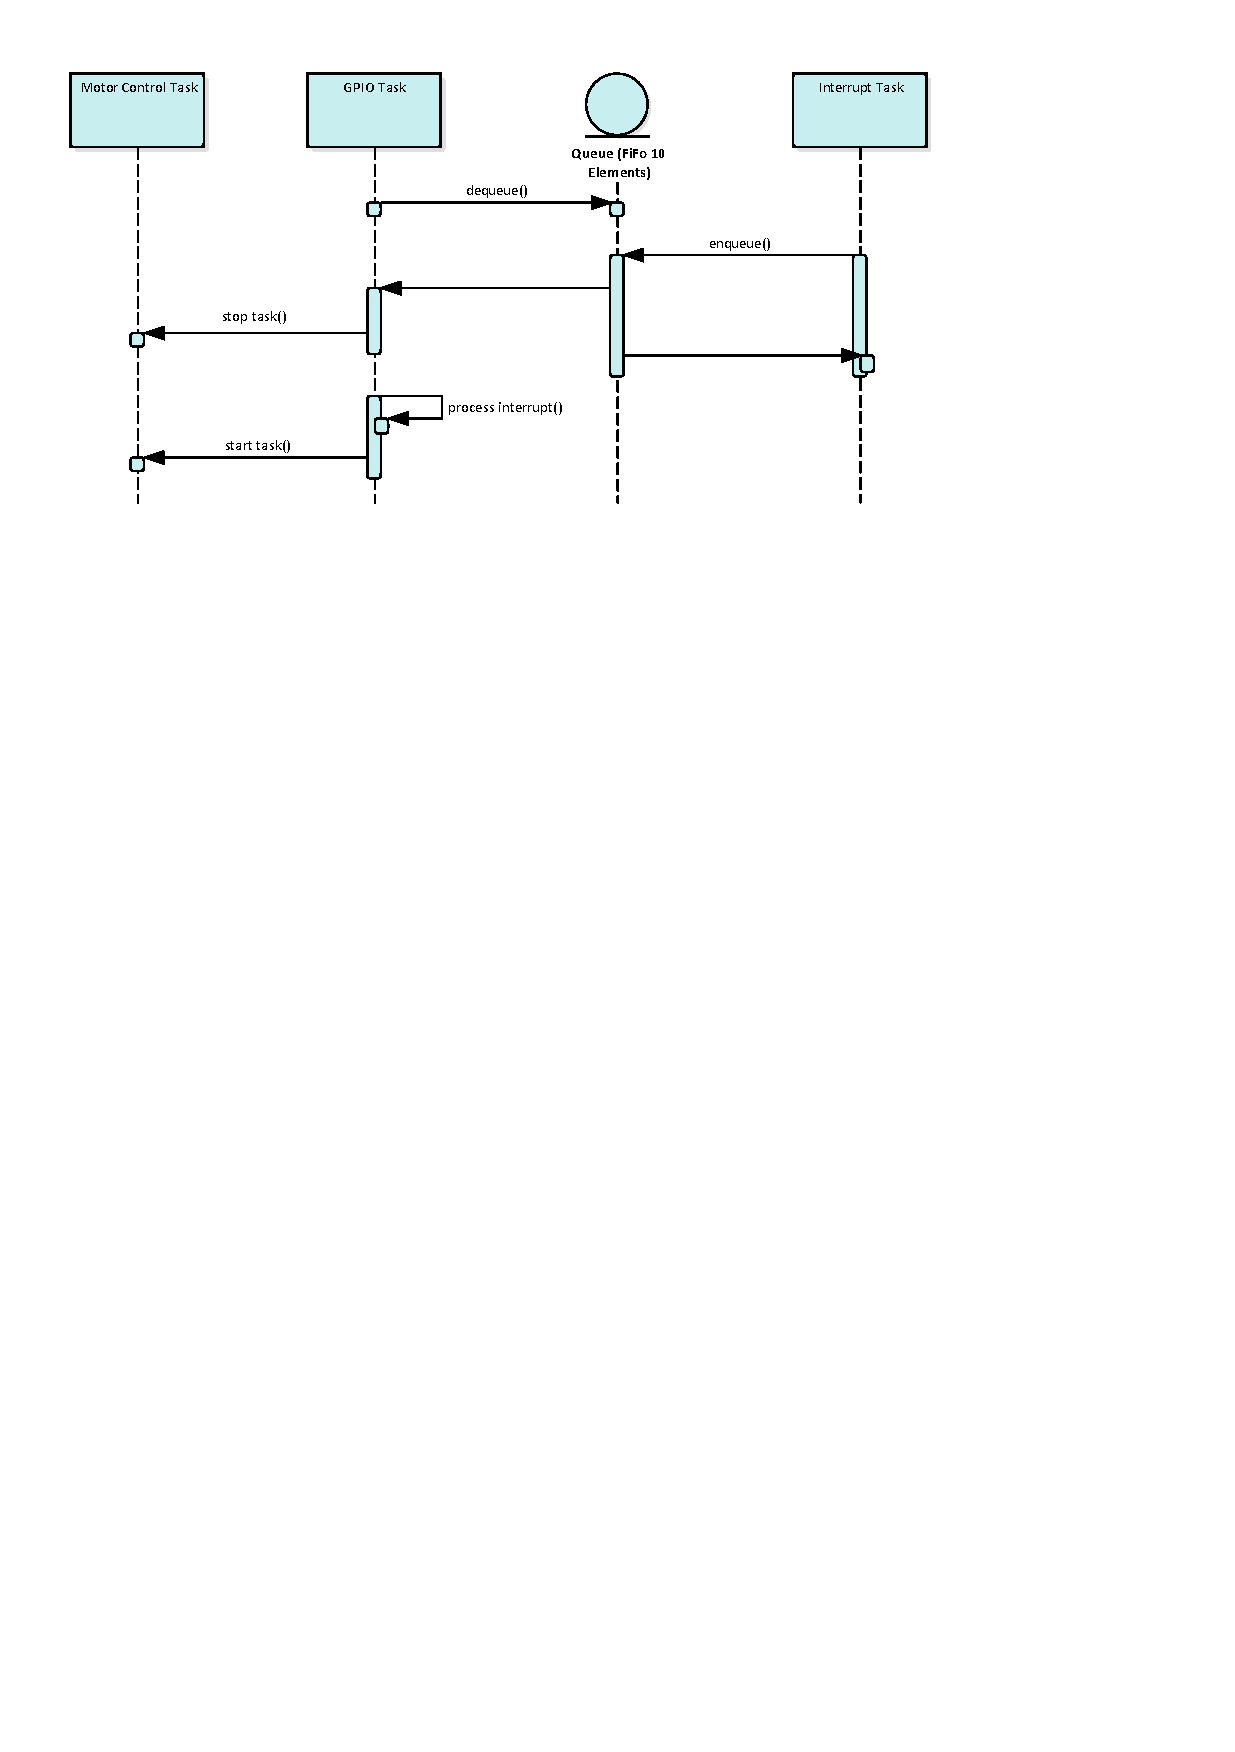
\includegraphics[width=1\linewidth]{images/Sequence_MotorControl}
	\caption[Sequence Diagramm MotorControl]{Sequenz Diagramm der Motorsteuerung}
	\label{fig:SequenceMotorControl}
\end{figure}

\begin{figure}[hbt]
	\centering
	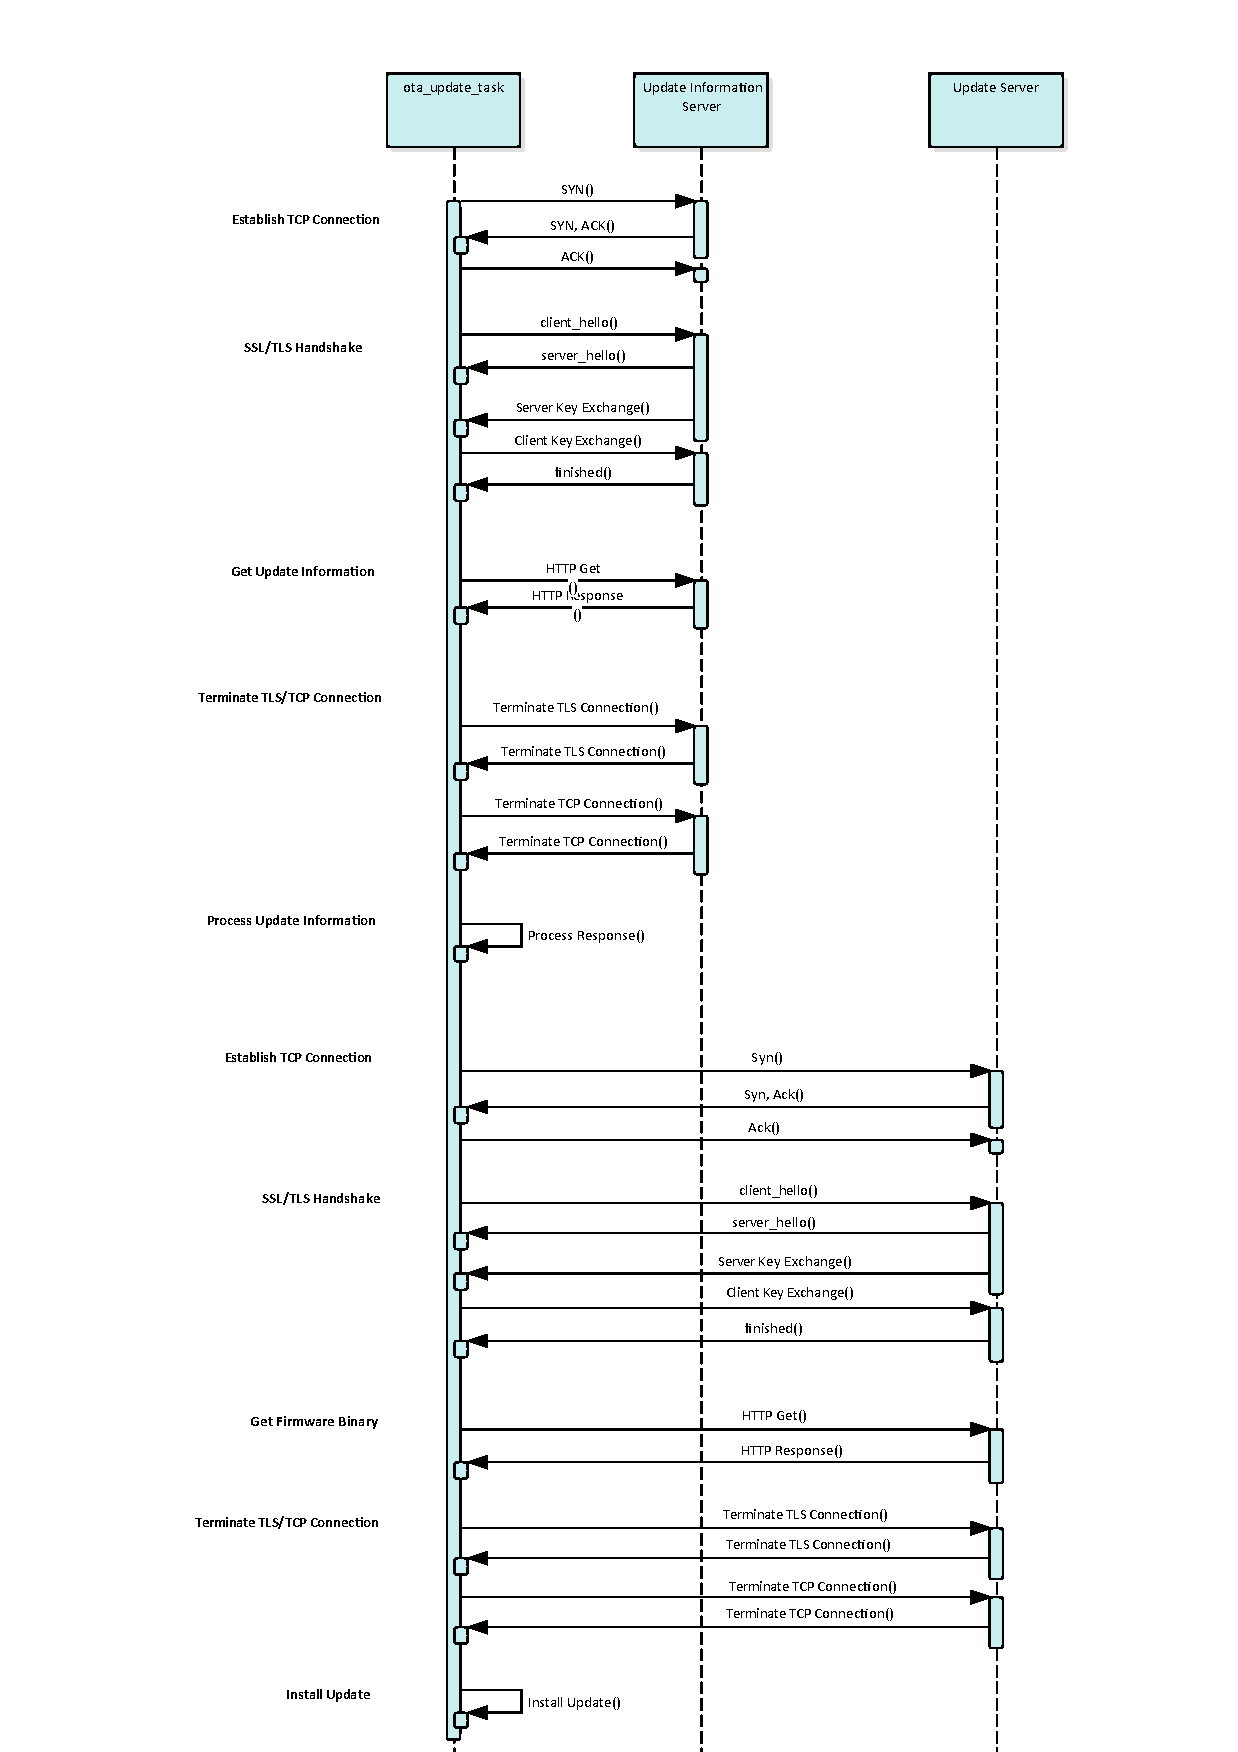
\includegraphics[width=0.7\linewidth]{images/Sequence_Update}
	\caption[Sequence_Update]{Sequenz Diagramm zum Ablauf eines Updates}
	\label{fig:Sequence_Update}
\end{figure}

\chapter{Implementierung}
\label{cha:Implementierung}

\section{Interessante Code-Segmente}

\section{Gegenüberstellung Komplexität (SLOC)}
% 1. Schätzung, 2.Schätzung, Lösung
\subsection{1. Schätzung}
Am Anfang der Projektplanung wurde davon ausgegangen, dass das Aktor Modul mit einem ESP32 realisiert wird. Für den zentralen Regler sollte ein Raspberry Pi verwendet werden, der gleichzeitig auch den MQTT Broker beinhaltet. Zusätzlich dazu sollte auf dem Raspberry Pi ein OpenThread Border Router eingerichtet werden. Dieser wäre für die Verbindung mit einem NRF52840 Mikrocontroller von Nordic Semiconductors gebraucht worden. Dieser Mikrocontroller sendet seine Daten mittels Low Power Bluetooth, was ihn extrem stromsparend macht. Mit einer 3V Batterie ist eine hohe Laufzeit erreichbar. Mit einem NRF Dongle wäre er mit dem Raspberry verbunden worden. Leider hatten wir mit diesem Mikrocontroller keine Erfahrung und mussten somit unsere Komponenten neu überdenken. Diesen Aufbau schätzten wir mit 2200 SLOC ab.
\subsection{2. Schätzung}
\label{cha:projektplanung_2schaetzung}
Da die Lösung mit dem NRF52840 Mikrocontroller später als zeitlich nicht realisierbar angesehen wurde, musste über einen Ersatz diskutiert werden. Da für das Aktor Modul bereits ein ESP32 verwendet wurde, lag es nahe, für das Sensormodul ebenfalls einen solchen Mikrocontroller zu verwenden. Der Vorteil war, dass viele Tasks des Empfängermoduls übernommen werden konnten. Beide Module unterschieden sich nur in ihren Aufgaben Tasks: Das Aktor Modul sollte eine Jalousie ansteuern, das Sensor Modul möglichst stromsparend Sensordaten einlesen und versenden.
\subsection{Finale Lösung}
Um die Einrichtung des Systems zu erleichtern, wurde zusätzlich zu dem Aufbau der 2. Schätzung aus Kapitel~\ref{cha:projektplanung_2schaetzung} ein Router verwendet, an den der Raspberry Pi als Regler mit LAN und die ESP32 Mikrocontroller des Sensor/Aktor Moduls mittels W-LAN angeschlossen wurden. Somit kann das BlindControl System an einen schon vorhandenen Router des Heimnetzwerkes gekoppelt werden. Mit dieser Lösung wurden 1540 SLOC benötigt. Die Kostenschätzung mittels COCOMOII\_2000.4 ist in Abbildung~\ref{fig:cost_end} dargestellt. Zusätzlich zu den 64h der Vorlesung wurden weitere 8h investiert. Damit ergibt sich im Schnitt 21 lines/h. 

Im Gegensatz zu der Schätzung in Kapitel~\ref{cha:Planung_cost} wurden 660 SLOC weniger benötigt, sowie 13 lines/h mussten weniger geschrieben werden.

\begin{figure}[hbt]
	\centering
	\includegraphics[width=1\linewidth]{images/cost_end_img}
	\caption[Kosten Realität]{Reale Kosten am Ende des Projekts.}
	\label{fig:cost_end}
\end{figure}
\chapter{Test}
\label{cha:Test}

\section{Test Procedure/Report}
Das Espressif IoT Development Framework (esp-idf) unterstützt von Haus aus unit tests mit dem Unity - unit test framework. Leider hat die Zeit nicht mehr ganz ausgereicht um entsprechende unit tests zu implementieren, da wir mit dem unity keine Erfahrung haben, wobei dies für die nähere Zukunft geplant ist. Aus diesem Grund wurden lediglich manuell die Funktion getestet, da dies durch die Anbindung an MQTT in Verbindung mit vielen Debug messages in der Anwendung recht einfach ist. Im Folgenden werden diese Tests der einzelnen Module in tabellarischer Form beschrieben.


\begin{longtable}[ht]{p{0.03\textwidth}  p{0.97\textwidth}}
	\captionabove[Test Sensor Module]{Test Sensor Module}\\
	\label{tab:sensortest}\\
	\toprule
	\rowcolor[HTML]{FFFC9E} 
	{\color[HTML]{333333} \textbf{Nr.}} & {\color[HTML]{333333} \textbf{Beschreibung}} \\* \midrule
	\endhead
	%
	1 & simulieren des Helligkeitssensors durch ein Potentiometer\\* \midrule
	2 & Prüfen ob Debugmessages zeigen dass der ESP32 nur bei entsprechender Helligkeitsänderung aufgeweckt wird\\* \midrule
	3 & Prüfen ob die entsprechende Nachricht auf das MQTT sensor topic gesendet werden \\*
	\bottomrule
\end{longtable}

\begin{longtable}[ht]{p{0.03\textwidth}  p{0.97\textwidth}}
	\captionabove[Regler Module]{Regler Module}\\
	\label{tab:reglertest}\\
	\toprule
	\rowcolor[HTML]{FFFC9E} 
	{\color[HTML]{333333} \textbf{Nr.}} & {\color[HTML]{333333} \textbf{Beschreibung}} \\* \midrule
	\endhead
	%
	1 & manuelle senden einer MQTT Nachricht mit einem Sensorwert\\* \midrule
	2 & Prüfen ob eine MQTT Nachricht mit der entsprechenden Positionsänderung gesendet wird\\* \midrule
	3 & manuelle senden einer MQTT Nachricht mit einer manuellen Positionsänderung\\* \midrule
	4 & Prüfen ob eine MQTT Nachricht mit der entsprechenden Positionsänderung gesendet wird und erst wieder nach 60 Minuten entsprechend von Sensorwerten gesteuert wird\\*
	\bottomrule
\end{longtable}

\begin{longtable}[ht]{p{0.03\textwidth}  p{0.97\textwidth}}
	\captionabove[Test Actuator Module]{Test Actuator Module}\\
	\label{tab:actuatortest}\\
	\toprule
	\rowcolor[HTML]{FFFC9E} 
	{\color[HTML]{333333} \textbf{Nr.}} & {\color[HTML]{333333} \textbf{Beschreibung}} \\* \midrule
	\endhead
	%
	1 & Senden einer entsprechend Formatierten MQTT Nachricht zur Ansteuerung der Jalousie auf verschiedene Positionen\\* \midrule
	
	2 & Prüfen ob Debugmessages zeigen dass eine entsprechende Ansteuerung vorgenommen wird\\* \midrule
	3 & manuelles triggern eines Interrupt Pins für die Endstopps\\* \midrule
	4 & Prüfen ob Debugmessages zeigen dass die Ansteuerung abgebrochen und die aktuelle Position auf die Position des Endstopps gesetzt wird\\*
	\bottomrule
\end{longtable}

\subsection{Testergebnis}
Alle beschriebenen Tests sind ohne Fehler durchlaufen worden.
\chapter{Installation/Benutzung}
\label{cha:Installation/Benutzung}

\section{Deployment Diagramm}

\begin{figure}[hbt]
	\centering
	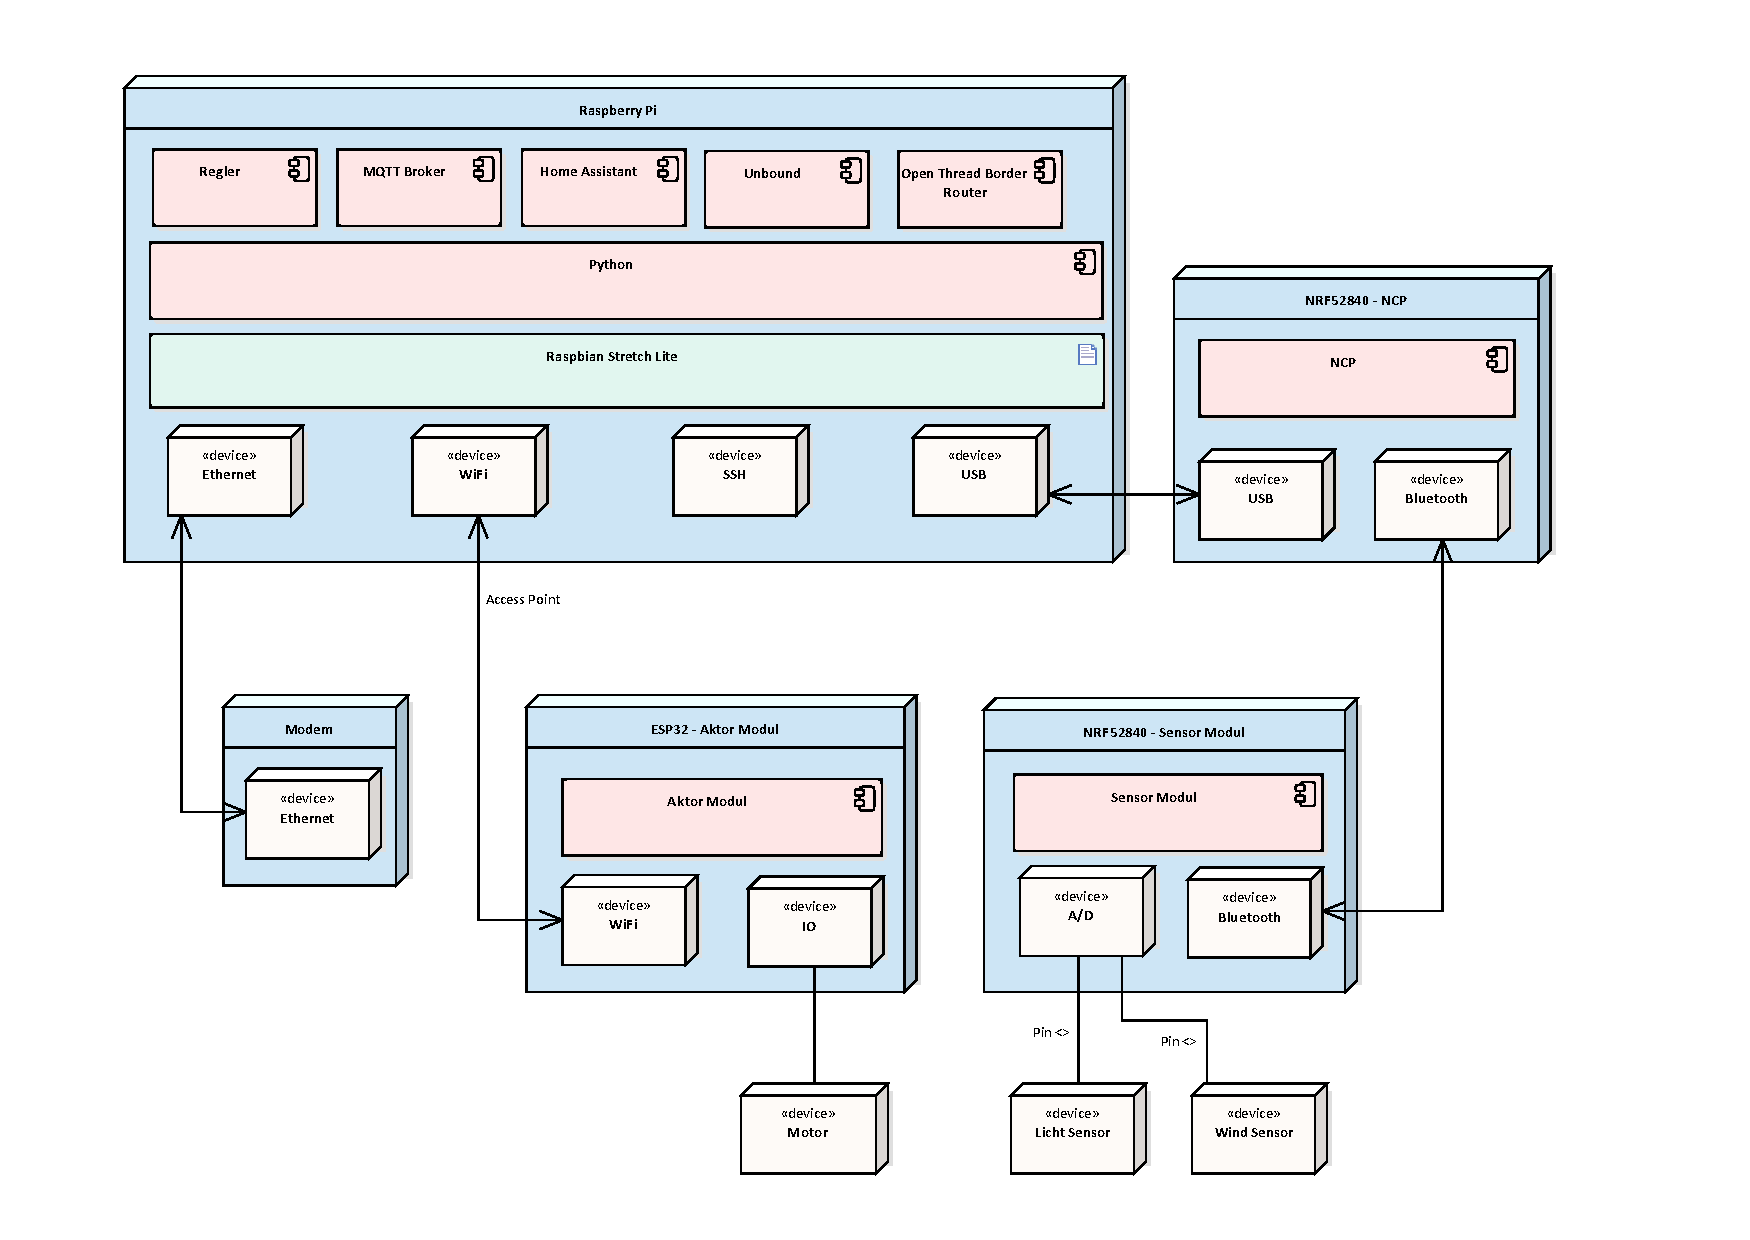
\includegraphics[width=1\linewidth]{images/Deployment}
	\caption[Deployment Diagramm]{Deployment Diagramm.}
	\label{fig:deployment_diagramm}
\end{figure}

Abbildung~\ref{fig:deployment_diagramm} zeigt das Deployment Diagramm des Systems. Im Folgenden wird einzeln auf die Installation der Module eingegangen.

\section{Sensor und Aktor Modul (ESP32)}
\label{cha:Installation_IDF}
\subsection{Schritt 1: Installation von Abhängigkeiten}
Um die ESP32 Mikrocontroller flashen zu können, muss zunächst das Espressif IoT Development Framework (ESP IDF)\nomenclature{ESP IDF}{Espressif IoT Development Framework} installiert und eingerichtet werden. An dieser Stelle sei auf die \href{https://docs.espressif.com/projects/esp-idf/en/latest/index.html}{Dokumentation von Espressif} hingewiesen, um die Programmierumgebung abhängig vom Betriebssystem richtig einzurichten. Weiterhin wird eine Installation von Git, sowie make benötigt.

\subsection{Schritt 1: Installation von Abhängigkeiten}
Der Quellcode für beide Module kann auf Github heruntergeladen werden: \href{https://github.com/maxbachmann-university/esp32-sensor-modul}{Sensor Modul}, \href{https://github.com/maxbachmann-university/esp32-actuator-module}{Aktor Modul}.

Zum Flashen des ESP32 gibt es entsprechende Makefiles, die den Vorgang vereinfachen. Einstellungen können mit \textbf{''make menuconfig''} vorgenommen werden. Die Abbildungen~\ref{fig:config_start} und ~\ref{fig:config_default} zeigen das Dialogfenster.
Interessante Einstellungsmöglichkeiten sind hier die Elemente:
\begin{itemize}
	\item \textbf{Security Features} um secure boot, sowie flash encryption zu aktivieren bzw. zu deaktivieren (Diese Einstellung sollte bei Unsicherheit besser deaktiviert bleiben, da sie in der Regel nicht umkehrbar ist)
	\item \textbf{Serial Flasher Config} Hier kann der serielle Port, an den der ESP32 angeschlossen ist, ausgewählt werden
	\item \textbf{Example Configuration} Hier können Projektspezifische Parameter wie die Verbindungsdaten des WLAN Routers, des MQTT Brokers und des OTA Servers angepasst werden
\end{itemize}

Im Folgenden sind die benötigten Befehle zum Flashen des ESP32 sowohl für das Sensor Modul, als auch für das Aktor Modul gelistet.
\lstset{caption={Installation des Sensor Moduls}}
\lstset{label={lst:rc.local}}
\begin{lstlisting}
git clone --depth=1 https://github.com/maxbachmann-university/esp32-sensor-modul
cd esp32-sensor-modul
make menuconfig		# Konfiguration vornehmen
make flash			# Flashen des esp32
\end{lstlisting}

\lstset{caption={Installation des Aktor Moduls}}
\lstset{label={lst:rc.local}}
\begin{lstlisting}
git clone --depth=1 https://github.com/maxbachmann-university/esp32-actuator-module
cd esp32-actuator-module
make menuconfig		# Konfiguration vornehmen
make flash			# Flashen des esp32
\end{lstlisting}

\begin{figure}[hbt]
	\centering
	\includegraphics[width=0.8\linewidth]{images/make_menuconfig_start}
	\caption[Konfiguration Startseite]{Startseite der Konfiguration.}
	\label{fig:config_start}
\end{figure}

\begin{figure}[hbt]
	\centering
	\includegraphics[width=0.8\linewidth]{images/make_menuconfig_default}
	\caption[Konfiguration Standard]{Default Werte der Konfiguration.}
	\label{fig:config_default}
\end{figure}

\section{Regler Modul (Raspberry PI)}

\subsection{Schritt 1: Installation von Raspbian}
Zunächst muss das image der aktuellsten Version von \href{https://www.raspberrypi.org/downloads/raspbian/}{Raspbian} auf die SD-Karte des Raspberry PI geladen werden.

\subsection{Schritt 2: MQTT Broker}
Im Grunde kann ein beliebiger MQTT Broker genutzt werden. Wir haben \href{http://mosquitto.org/}{Mosquitto} benutzt. Dieser Broker kann mit dem Befehl in Listing~\ref{lst:installmosquitto} installiert werden und läuft sofort.

\lstset{caption={Installation von Mosquitto.}}
\lstset{label={lst:installmosquitto}}
\begin{lstlisting}
sudo apt install -y mosquitto mosquitto-clients
\end{lstlisting}

\subsection{Schritt 3: Hinzufügen des Python Skripts}
Für die Regelung wird ein \href{https://github.com/maxbachmann-university/blind-controller}{Python Skript} verwendet, welches auch auf Github zu finden ist. Dieses kann in einem beliebigen Ort auf dem Raspberry Pi gespeichert werden, inklusive der ''config.yml'' Datei. In dieser können die Zugangsdaten zu dem MQTT Broker angepasst werden. Für den Autostart des Skripts beim Neustart, muss mit Hilfe des Befehls wie in Listing~\ref{lst:rc.local} im Terminal der Texteditor der Datei ''rc.local'' aufgerufen werden. Anschließend wird die Datei vor der Zeile ''exit 0'' um eine weitere Zeile ergänzt, in die nach einem ''python'' der Pfad zu dem Python Skript angegeben wird, gefolgt von einem ''\&''. Das ganze sieht dann zum Beispiel so aus, wie in Listing~\ref{lst:autostart}.

\lstset{caption={Öffnen der Autostart Datei im Editor Nano.}}
\lstset{label={lst:rc.local}}
\begin{lstlisting}
sudo nano /etc/rc.local
\end{lstlisting}

\lstset{caption={Anpassung der Autostart Datei.}}
\lstset{label={lst:autostart}}
\lstset{language=Python}
\begin{lstlisting}
python3 /home/pi/controller.py &
exit 0
\end{lstlisting}
\chapter{Benutzerhandbuch}
\label{cha:Benutzerhandbuch}
% Was auch immer hier hin kommt...
% Auf jeden Fall ein Verweis auf das Github Wiki :D
\chapter{Fazit und Ausblick}
\label{cha:Fazit und Ausblick}

Der Aktuelle Stand ist zwar grundsätzlich betriebsbereit, wobei gegebenenfalls einige Anpassungen an die individuellen Gegebenheiten nötig ist. Dies betrifft sowohl die Helligkeitsmessung, da hier aktuell noch nicht getestet ist, ob hier die Helligkeitsstärken tatsächlich sinnvoll sind, als auch die Ansteuerung der Jalousie, da hier aktuell von einem bestimmten Schrittmotortreiber ausgegangen wird, wobei sich dies von Jalousie zu Jalousie unterscheiden kann. Das Regler Module besitzt bereits die Funktion getrennt mehrere Räume anzusteuern, wobei sowohl das Sensor Module, als auch das Actuator Module hiervon aktuell noch keinen Gebrauch machen. Insbesondere die Sicherheitsvorkehrungen die leider bei vielen IOT Projekten gänzlich vernachlässigt werden, sind bei dieser Realisierung jedoch bereits sehr gut, wobei leider aktuell noch ein eigener "Update Server" nötig ist auf den die binaries für OTA Updates abgelegt werden. Durch den modularen Aufbau lässt sich ein Großteil des Projektes auch auf andere IOT Geräte anwenden (Insbesondere die MQTTS Funktionalität und die OTA Updates).

Aus den oben genannten Gründen soll sich das Projekt in Zukunft auch mehr auf die Aspekte der sicheren Kommunikation und Updatefähigkeit von IOT Geräte konzentrieren um diese in anderen Projekten nur noch als Teilkomponenten einfügen zu müssen. Konkret sind hier für die nähere Zukunft folgende Erweiterung geplant:

\begin{itemize}
	\item Da der Code sowieso öffentlich auf Github zur Verfügung gestellt wird soll das Deployment mithilfe einer Continous Integration (CI) automatisiert werden, so dass die aktuellste binary als release zur Verfügung gestellt wird, wobei diese dann auch direkt für OTA Updates genutzt werden können.
	\item Die aktuellen Tests sollen automatisiert werden, so dass diese durch eine CI beispielsweise vor Updates des aktuellen Produktionscode möglich sind
	\item Aktuell muss der Nutzer noch selbst einen MQTT Broker aufsetzten mit TLS und username/password Authentification. Weiterhin muss er selbst entsprechende Skripte wie das Regler Module in diesem Projekt starten. Dieser Prozess soll in Zukunft automatisiert werden um so auch Personen ohne das nötige technische Hintergrundwissen eine einfache Installation zu ermöglichen
	\item Die Unterstützung von mehreren Räumen soll auf den MQTT Task ausgeweitet werden um so Projekten direkt eine einfache Möglichkeit zur Ansteuerung von Geräten in verschiedenen Räumen zu geben
\end{itemize}

Weitere Erweiterungen sind in vielfältiger Art und Weise möglich, wobei die eben genannten aktuell die höchste Priorität besitzen.

% ---- Literaturverzeichnis ----------

% \bibliography{literature/literatur1,literature/literatur2}
										% Einbindung mehrerer Verzeichnisse in einem \bibliography Befehl mit Kommata trennen - keine Leerzeichen nach den Kommata!
\bibliographystyle{alphadin}           	%plain: alphabetisch, unsrt: nach Zitat, alphadin: NameJahr


% -----Ausgabe aller Verzeichnisse ---
\setlength{\parskip}{0.5\baselineskip}
%\renewcommand{\indexname}{Sachwortverzeichnis}
%\printindex								% Erzeugen des Indexverzeichnises
%\addcontentsline{toc}{chapter}{\indexname}
% Version 0.1 vom 31.10.14 - T. Kibler

% Änderungswünsche bitte an T. Kibler melden

% alle Abkürzungen, die in der Arbeit verwendet werden. Nachfolgend sind allgemeine Abkürzungen aufgelistet. Die für die Arbeit spezifischen Abkürzungen sollten innerhalb des Haupttextes aufgeführt werden. Die Alphabetische Sortierung übernimmt Latex.

\nomenclature{Abb.}{Abbildung}
\nomenclature{bzw.}{beziehungsweise}
\nomenclature{DHBW}{Duale Hochschule Baden-Württemberg}
\nomenclature{ebd.}{ebenda}
\nomenclature{et al.}{at alii}
\nomenclature{etc.}{et cetera}
\nomenclature{evtl.}{eventuell}
\nomenclature{f.}{folgende Seite}
\nomenclature{ff.}{fortfolgende Seiten}
\nomenclature{ggf.}{gegebenenfalls}
\nomenclature{Hrsg.}{Herausgeber}
\nomenclature{Tab.}{Tabelle}
\nomenclature{u. a.}{unter anderem}
\nomenclature{usw.}{und so weiter}
\nomenclature{vgl.}{vergleiche}
\nomenclature{z. B.}{zum Beispiel}
\nomenclature{z. T.}{zum Teil}				% Datei mit allgemeinen Abkürzungen laden
\renewcommand{\nomname}{Verzeichnis verwendeter Formelzeichen und Abkürzungen}
\setlength{\nomlabelwidth}{.20\hsize}
\renewcommand{\nomlabel}[1]{#1 \dotfill}
\setlength{\nomitemsep}{-\parsep}
\printnomenclature						% Erzeugen des Abkürzungsverzeichnises, siehe auch Inhalt der Datei pages/abkuerzungen.tex
\cleardoublepage
%\renewcommand{\glossaryname}{Glossar}
%\printglossaries
%\cleardoublepage
\listoffigures 							% Erzeugen des Abbildungsverzeichnisses 
\cleardoublepage
\listoftables 							% Erzeugen des Tabellenverzeichnisses
\cleardoublepage

% -----Anhang ------------------------

\begin{appendix}
\clearpage
%\pagenumbering{Roman}					% große, römische Seitenzahlen für Anhang, falls gewünscht
%\addchap{Anhang im Zip Archiv}
\setcounter{chapter}{1}
\setcounter{section}{0}
\setcounter{table}{0}
\setcounter{figure}{0}

\begin{itemize}
	\item README
	\item Blind Controller (Ordner mit Quellcode)
	\item Sensor Modul (Ordner mit Quellcode)
	\item Aktor Modul (Ordner mit Quellcode)
\end{itemize}
%\addchap{Anhang E}
\setcounter{chapter}{5}
\setcounter{section}{0}
\setcounter{table}{0}
\setcounter{figure}{0}

\section{Wichtige \LaTeX -Befehle}

\begin{tabbing}
\hspace*{0cm} \= \hspace{0.25\linewidth} \= \+\kill
\textbackslash \textit{label}\{\}	\> Definition eines Labels, auf welches referenziert werden kann\\ 
	\> z.B.: \textbackslash \textit{label}\{fig:MyImage\}\\ 
\textbackslash \textit{ref}\{\}	\> Setzen einer Referenz zu einem Label\\
\textbackslash \textit{pageref}\{\}	\> Gibt die Seitenzahl zu einer Referenz zurück\\
	\> z.B.: Tabelle\~{}\textbackslash \textit{ref}\{tab:messdaten\} fasst die Messergebnisse zusammen.\\ 
\textbackslash \textit{cite}\{\}	\> Literaturreferenz einfügen\\
\textbackslash \textit{cite}[S. x]\{\}	\> Literaturreferenz mit Angabe einer Seitenzahl \glqq x\grqq~einfügen\\

\textbackslash \textit{footnote}\{\}	\> Fußnote einfügen\\ 
\~{}	\> Einfügen eines geschützten Leerzeichens\\ 
\textdollar \textit{Formel} \textdollar	\> Eingabe einer Formel im Text\\
\textbackslash \textit{nomenclature}\{a.\}\{ab\}	\> Aufnahme der Abkürzung \glqq a.\grqq~für \glqq ab\grqq~in das Abkürzungsverzeichnis.\\
\textbackslash \textit{index}\{Obst!Birne\} \> Aufnahme des Begriffs \glqq Birne\grqq~in den Index unter \glqq Obst\grqq. \index{Obst!Birne} \\
\textbackslash \textit{clearpage}	\> Ausgabe aller Gleitobjekte und Umbruch auf neue Seite\\ 
\end{tabbing}

\clearpage

\section{Vorlagen für \LaTeX Umgebungen}

\subsection{Listen und Aufzählungen}

Es gibt folgende Listentypen. Die wichtigsten:

\begin{itemize}
	\item Einfache Liste mit \textit{itemize}-Umgebung
	\item ...
\end{itemize}

\begin{enumerate}
	\item Nummerierte Liste mit \textit{enumerate}-Umgebung
	\item ...
\end{enumerate}

\begin{enumerate}[label=\alph*.]
	\item wobei man bei der \textit{enumerate}-Umgebung leicht die Art der Numerierung ändern kann,
	\item ...
\end{enumerate}

und durch verschachtelte Umgebungen verschiedene Aufzählungsebenen darstellen kann:

\begin{enumerate}[label=\alph*)]
	\item Erster Aufzählungspunkt der ersten Ebene
	\item ...
	\begin{itemize}
		\item Erster Punkt der zweiten Ebene
		\item Zweiter Punkt der zweiten Ebene
	\end{itemize}
	\item Das sollte an Beispielen zunächst einmal genügen.
\end{enumerate}

\clearpage

\subsection{Bilder und Grafiken}

Bilder können als PDF-, JPG-, und PNG-Bilder in \LaTeX eingebunden werden. Damit eine Grafik in hoher Qualität dargestellt wird, sollte das Dateiformat der Grafik vektorbasiert sein, d.h. als PDF-Datei vorliegen. Viele Zeichenprogramme unterstützen einen PDF-Export (z.B. GIMP, Adobe Illustrator, etc.). Für Grafiken aus PowerPoint sei folgende Vorgehensweise beim Export empfohlen:

\begin{enumerate}
	\item Die gewünschte Grafik in PowerPoint zeichnen.
	\item Gewünschten Bildbereich markieren, rechte Maustaste klicken und \glqq Als Grafik speichern ...\grqq~wählen.
	\item Grafik im Format EMF abspeichern. Das EMF-Format ist vektorbasiert.\footnote{Mit dem Mac kann in PowerPoint die Grafik direkt im PDF-Format exportiert werden. Die weiteren Schritte entfallen daher.}
	\item Mit dem Programm XnView die Grafik im EMF-Format in PDF wandeln und abspeichern.
	\item Die so erzeugte PDF-Datei enthält eine vektorbasierte Grafik und kann in \LaTeX eingebunden werden.
\end{enumerate}

Abbildung~\ref{fig:MyImage} zeigt ein Beispielbild einer Grafik, welche aus PowerPoint exportiert wurde.

\begin{figure}[hbt]
	\centering
	
\includegraphics[width=0.3\linewidth]{images/MyImage}
	\caption[Beispiel für die Einbindung eines Bildes.]{Beispiel für die Einbindung eines Bildes (PDF-, JPG-, und PNG-Bilder können eingebunden werden).}
	\label{fig:MyImage}
\end{figure}

Der Quellcode des Beispielbildes aus Abbildung~\ref{fig:MyImage} ist in Listing~\ref{lst:fig} zu sehen.

\begin{lstlisting}[caption=Quellcode der Abbildung~\ref{fig:MyImage}.,label=lst:fig]
\begin{figure}[hbt]				% here, bottom, top
\centering						% Zentrierung

\includegraphics[width=0.6\linewidth]{images/MyImage}		
\caption[Beispiel für die Einbindung eines Bildes.]{Beispiel für die Einbindung eines Bildes (PDF-, JPG-, und PNG-Bilder können eingebunden werden).}
\label{fig:MyImage}
\end{figure}
\end{lstlisting}

\clearpage

Grafiken mit Tikz werden mit dem \textit{input}-Befehl in die \textit{figure}-Umgebung geladen:

\begin{figure}[hbt]
	\centering
	\begin{tikzpicture}
		\begin{axis}[scale=1.3,legend entries={Messwerte mit Fehlerbalken,
			$\pgfmathprintnumber{\pgfplotstableregressiona} \cdot x  
			\pgfmathprintnumber[print sign]{\pgfplotstableregressionb}$}, legend style={draw=none},legend style={at={(0.01,0.98)},anchor=north west},xlabel=Stromstärke $I \; \mathrm{ \lbrack mA \rbrack}$,ylabel=Spannung $U \; \mathrm{ \lbrack V \rbrack}$]
		\addlegendimage{mark=*,blue}
		\addlegendimage{no markers,red}
\addplot+[error bars/.cd, y dir=both,y explicit]
table[x=x,y=y,y error=errory] 
{pgfplot/messdaten_mitfehler.dat};
\addplot table[mark=none,y={create col/linear regression={y=y}}]
{pgfplot/messdaten_mitfehler.dat};
	\end{axis}
\end{tikzpicture}
	\caption[Diagramm, erstellt mit dem \textit{pgfplot}-Befehlssatz.]{Ein Diagramm, erstellt in der \textit{tikzpicture}-Umgebung mit dem \textit{pgfplot}-Befehlssatz. Das Diagramm stellt Messdaten, deren Fehlerbalken und eine Regressionskurve dar. Die Messdaten werden von einer separaten Datei eingelesen und die Regressionskurve wurde mit \textit{pgfplot} berechnet und erstellt.}
	\label{fig:pgfplot}
\end{figure}

Auch hierzu der Quellcode in Listing~\ref{lst:pgfplot}, in Listing~\ref{lst:tikz} ist der Quellcode der Datei \textit{mess\_fehlerbalken.tex} dargestellt.

\begin{lstlisting}[caption=Quellcode der Abbildung~\ref{fig:pgfplot}.,label=lst:pgfplot]
\begin{figure}[hbt]
\centering
\begin{tikzpicture}
		\begin{axis}[scale=1.3,legend entries={Messwerte mit Fehlerbalken,
			$\pgfmathprintnumber{\pgfplotstableregressiona} \cdot x  
			\pgfmathprintnumber[print sign]{\pgfplotstableregressionb}$}, legend style={draw=none},legend style={at={(0.01,0.98)},anchor=north west},xlabel=Stromstärke $I \; \mathrm{ \lbrack mA \rbrack}$,ylabel=Spannung $U \; \mathrm{ \lbrack V \rbrack}$]
		\addlegendimage{mark=*,blue}
		\addlegendimage{no markers,red}
\addplot+[error bars/.cd, y dir=both,y explicit]
table[x=x,y=y,y error=errory] 
{pgfplot/messdaten_mitfehler.dat};
\addplot table[mark=none,y={create col/linear regression={y=y}}]
{pgfplot/messdaten_mitfehler.dat};
	\end{axis}
\end{tikzpicture}
\caption[Diagramm, erstellt mit dem \textit{pgfplot}-Befehlssatz.]{Ein Diagramm, erstellt in der \textit{tikzpicture}-Umgebung mit dem \textit{pgfplot}-Befehlssatz. Das Diagramm stellt Messdaten, deren Fehlerbalken und eine Regressionskurve dar. Die Messdaten werden von einer separaten Datei eingelesen und die Regressionskurve wurde mit \textit{pgfplot} berechnet und erstellt.}
\label{fig:pgfplot}
\end{figure}
\end{lstlisting}

\begin{lstlisting}[caption=Quellcode der Datei \textit{mess\_fehlerbalken.tex}.,label=lst:tikz]
\begin{tikzpicture}
\begin{axis}[scale=1.3,legend entries={Messwerte mit Fehlerbalken,
$\pgfmathprintnumber{\pgfplotstableregressiona} \cdot x  
\pgfmathprintnumber[print sign]{\pgfplotstableregressionb}$}, legend style={draw=none},legend style={at={(0.01,0.98)},anchor=north west},xlabel=Stromstärke $I \; \mathrm{ \lbrack mA \rbrack}$,ylabel=Spannung $U \; \mathrm{ \lbrack V \rbrack}$]
\addlegendimage{mark=*,blue}
\addlegendimage{no markers,red}
\addplot+[error bars/.cd, y dir=both,y explicit]
table[x=x,y=y,y error=errory] 
{pgfplot/messdaten_mitfehler.dat};
\addplot table[mark=none,y={create col/linear regression={y=y}}]
{pgfplot/messdaten_mitfehler.dat};
\end{axis}
\end{tikzpicture}
\end{lstlisting}

\clearpage

\subsection{Tabellen}

\begin{table}[hbt]	
	\centering
	\renewcommand{\arraystretch}{1.5}	% Skaliert die Zeilenhöhe der Tabelle
	\captionabove[Liste der verwendeten Messgeräte]{Liste der verwendeten Messgeräte. Die Genauigkeitsangaben beziehen sich auf die Standardabweichung $1\cdot \sigma$.}
	\label{tab:bsp}
	\begin{tabular}{ccccc}
		\textbf{Messgerät} & \textbf{Hersteller} & \textbf{Typ} & \textbf{Verwendung} & \textbf{Genauigkeit}\\ 
		\hline 
		\hline 
		\parbox[t]{0.2\linewidth}{\centering Spannungs-\\versorgung} & Voltmaker & HV2000 & \parbox[t]{0.2\linewidth}{\centering Spannungs-\\versorgung der\\Platine} & $\Delta U = \pm 5 $~mV \\ % Der parbox-Befehl ist erforderlich, damit ein Zeilenumbruch erzeugt werden kann. c-Spalten (zentriert) erlauben nicht automatisch einen Zeilenumpruch. Linksbündig gesetzte p-Spalten erlauben automatisch den Zeilenumbruch.
		Strommessgerät & Currentcount & Hotamp 16 & \parbox[t]{0.2\linewidth}{ \centering Strommessung\\am Versorgungspin\\des µC} & $\Delta I = \pm 0.1$~A \\ 
		\hline 
	\end{tabular} 
\end{table}

Der Quellcode der Beispieltabelle~\ref{tab:bsp} ist in Listing~\ref{lst:tab} zu sehen.

\begin{lstlisting}[caption=Quellcode der Tabelle~\ref{tab:bsp}.,label=lst:tab]
\begin{table}[hbt]	
\centering
\renewcommand{\arraystretch}{1.5}	% Skaliert die Zeilenhöhe der Tabelle
\captionabove[Liste der verwendeten Messgeräte]{Liste der verwendeten Messgeräte. Die Genauigkeitsangaben beziehen sich auf die Standardabweichung $1\cdot \sigma$.}
\label{tab:bsp}
\begin{tabular}{ccccc}
\textbf{Messgerät} & \textbf{Hersteller} & \textbf{Typ} & \textbf{Verwendung} & \textbf{Genauigkeit}\\ 
\hline 
\hline 
\parbox[t]{0.2\linewidth}{\centering Spannungs-\\versorgung} & Voltmaker & HV2000 & \parbox[t]{0.2\linewidth}{\centering Spannungs-\\versorgung der\\Platine} & $\Delta U = \pm 5 $~mV \\ % Der parbox-Befehl ist erforderlich, damit ein Zeilenumbruch erzeugt werden kann. c-Spalten (zentriert) erlauben nicht automatisch einen Zeilenumpruch. Linksbündig gesetzte p-Spalten erlauben automatisch den Zeilenumbruch.
Strommessgerät & Currentcount & Hotamp 16 & \parbox[t]{0.2\linewidth}{ \centering Strommessung\\ am Versorgungspin\\ des \textmu C} & $\Delta I = \pm 0.1$~A \\ 
\hline 
\end{tabular} 
\end{table}
\end{lstlisting}

\clearpage

\subsection{Formeln}

Formeln lassen sich in \LaTeX~ganz einfach schreiben. Es gibt unterschiedliche Umgebungen zum Schreiben von Formeln. Z.B. direkt im Text $v=s/t$ oder abgesetzt

\[F=m \cdot a\]

oder auch, wie in wissenschaftlichen Dokumenten üblich, nummeriert

\begin{equation}
P=\frac{U^2}{R} \quad .
\label{eqn:leistung}
\end{equation}

Mit einem Label in Formel~\ref{eqn:leistung} lassen sich natürlich auch Formeln im Text referenzieren. \LaTeX~verwendet im Formelmodus einen eigenen Schriftsatz, welcher entsprechend der gängigen Konventionen kursive Zeichen verwendet. Sollen im Formelmodus Einheiten in normaler Schriftart eingefügt werden, dann kann dies über den Befehl \textbackslash \textit{mathrm}\{\} erwirkt werden, wie im Quellcode von Formel~\ref{eqn:leistungMitEinh} zu sehen ist.

\begin{equation}
P=\frac{U^2}{R} = \frac{\left( 100~\mathrm{V}\right)^2}{100~\Omega} = 100~\mathrm{W}\quad .
\label{eqn:leistungMitEinh}
\end{equation}

Zum direkten Vergleich sind die Einheiten in Formel~\ref{eqn:leistungMitEinhfalsch} falsch dargestellt:

\begin{equation}
P=\frac{U^2}{R} = \frac{\left( 100~V\right)^2}{100\,\varOmega} = 100\,W
\label{eqn:leistungMitEinhfalsch}
\end{equation}

Das sind nur ein paar wenige Beispiele und es gibt sehr viele Packages, um Besonderheiten in Formeln realisieren zu können, z.B. mehrzeilige Formeln mit vertikaler Ausrichtung. Nennen Sie Formeln nur, wenn diese zum besseren Verständnis auch wirklich nützlich sind.

Folgende Befehle sind innerhalb von Formel-Umgebungen nützlich:
\begin{tabbing}
	\hspace*{0cm} \= \hspace{0.35\linewidth} \= \+\kill
	\textbackslash \textit{text}\{\}	\> Damit kann in Formel-Umgebung Text geschrieben werden.\\ 
	\textbackslash, \textbackslash: \textbackslash; oder \textbackslash quad und \textbackslash qquad \> Zusätzlichen Abstand zwischen Symbolen einfügen.\\
	\textbackslash \textit{notag} \> Nummerierung einer bestimmten Formel ausschalten.
\end{tabbing}

Abschließend nochmals ein kleines Beispiel:

\begin{eqnarray}
\sum\limits_{n=1}^\infty f\left(x_n\right)\cdot \Delta x=  \lim\limits_{\Delta x \rightarrow 0} \frac{f\left(x_0+\Delta x\right)-f\left(x_0\right)}{\Delta x} = \frac{\diff f}{\diff x} = \dot{f}(x)
\end{eqnarray}		% Zeile auskommentieren bei finalem Dokument!
\end{appendix}


\end{document}